\documentclass{article}

\usepackage{graphicx}
\usepackage{amsmath,amsthm,amsfonts}                % AMS Math
\usepackage{thmtools}                                       % Theorem Tools
\usepackage{bbm}                                             % Bold Math


\title{Assignment 3}
\author{Ming Liang Ang}
\date{May 2022}

\begin{document}

\maketitle

\section{Question 1}
In the question, we are given a complex number $c$ and the inital value $z = 0$, we can generate the sequence by iterating $z=z*z +c$ until the maximum number of iterations is reached or until the 
point where its modulus is larger than a threshold (i.e at that point it diverges) in order to get a set of values of $c$ where the sequence diverege. 
\\\\
For the first part of the question, we return $0$ if the at the point $c$ the sequences divereges (i.e outside the threshold) and $1$ othewrise to make an image in which your points c that diverge
are given one color and those that stay bounded are given another.
\\\\

\includegraphics[width=\textwidth]{mandelbrot1.png}
\\\\
For the second part of the question, we return the number of iterations it takes the sequence to get larger than the threshold (i.e the point at which it diverges) to make the second image where the points
are coloured by a colourscale that indicates the iteration number at which the given point diverged
\\\\
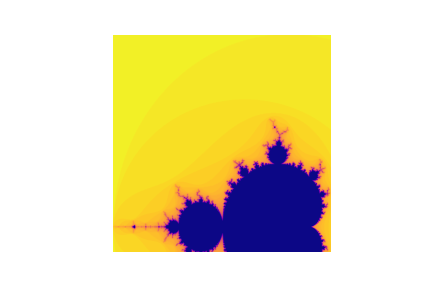
\includegraphics[width=\textwidth]{mandelbrot2.png}
\newpage
\section{Question 2}
In the first two parts of the question, we first define a function for each of the derivatives of $X, Y, Z$ to code up the equation and then use scipy function to solve the inital value problem of the ODE. For the third part, in order to reproduce figure 1 we use part 2 to get the numerical solution of the equations for first 1000 iterations (repersenting the top graph), the second 1000 iterations (repersenting the middle graph) and third 1000 iterations (repersenting the bottom graph).
\\\\
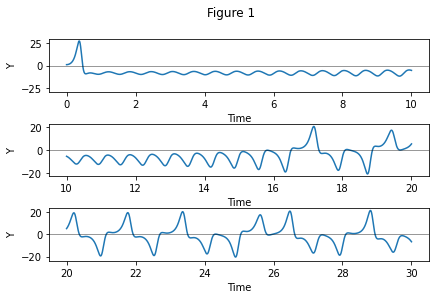
\includegraphics[width=\textwidth]{figure1.png}
\newpage
\noindent
For the fourth part of the question, we use the second part of the question to get the numerical solution of the equations then project on the $X-Y$, $Y-Z$ plane in the phase space of the segement of the trajectory extending from iteration 1400 to 1900. 
\\\\
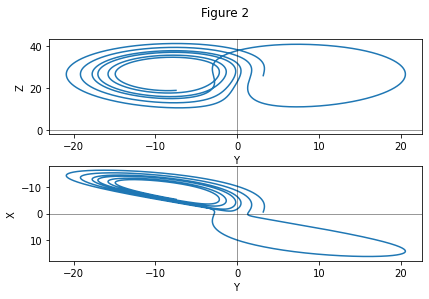
\includegraphics[width=\textwidth]{figure2.png}
\newpage
\noindent
For the final part of the question, we solve the ODE for the initial conditions $W_0$ and $W'_0$ and then compute the euclidean distance between the 2 solutions. 
\\\\
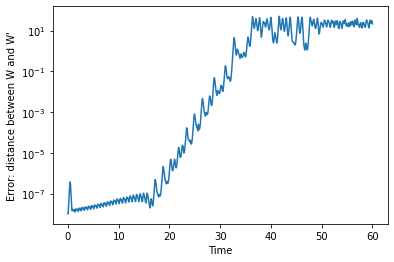
\includegraphics[width=\textwidth]{error.png}
\end{document}